\section{External devices}

Your third and last approac was to use an external devices to monitor and measure the context switching time.

Our first idea was to implement it with Python3.7 on a desktop computer.
Using the UART protocol over USB, the board sends a single byte containing the thread ID that is read by a Python script on the computer.

The motivations for using this alternative are:
\begin{itemize}
  \item Sending one byte of data over USB with UART have a smaller impact than computing the context switching time locally on the board;
  \item Heavy computational tasks of the framework are done on the computer and not on the board;
  \item Using Python3.7, we can achieve a time precision at the nanosecond.
\end{itemize}

However, after discussing with the embedded community, we abandonned this idea for the following reasons.
There is buffering happening on the USB-serial chip on the board, on the PC's USB hardware, in the PC USB-serial driver and also in the desktop operating systems.
Those buffering will add delay in our measurements.
Context switchs will occur on the desktop computer that will invalidate any timing value.

Instead, we decided to use a device called the Pocket Science Lab to perform our experiment.

\begin{figure}[!ht]
  \centering
  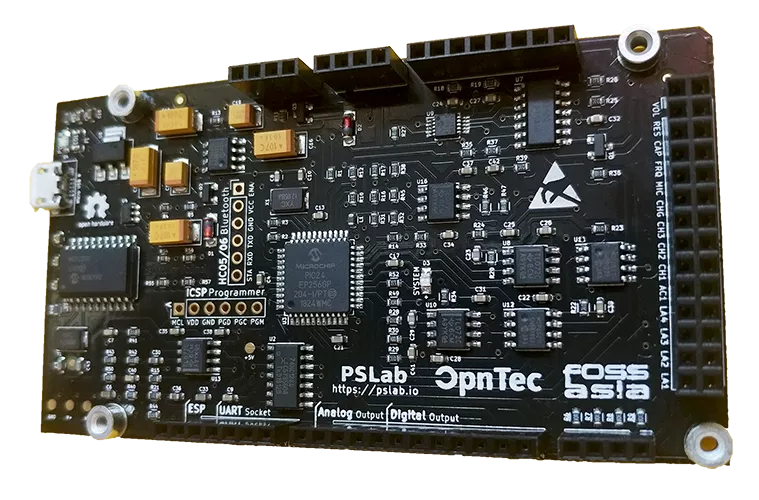
\includegraphics[scale=0.25]{assets/pslab.png}
  \caption{\label{fig:pslab}Pocket Science Lab device from \href{https://pslab.io}{PSLab.io}}
\end{figure}

The Pocket Science Lab device from \href{https://pslab.io}{PSLab.io} comes with a built-in 4-Channel up to 2MSPS oscilloscope, multimeter, 4-Channel, 4 MHz logic analyser, and other digital instruments.
Using the Python librairy \href{https://github.com/fossasia/pslab-python}{pslab-python}, we can communicate with the board and experiment with it.

The PSLab will monitor a single GPIO and measure the context switching time from it.
The figure \ref{fig:external-framework-context-switching-time-measurement} shows the steps in the measurement with the PSLab.
Each task will set the GPIO up at the start of its execution and then reset the GPIO once it ended.
In our example, the task 1 set up the GPIO at the step A and the GPIO is in high position at step A'.
Once the task 1 is finished, it reset the GPIO at the step B that will be in position at step B'.
The same process occurs for the task 2.
The task 2 set up the GPIO at step C.
The GPIO is in high position at step C'.
Finally, the task 2 reset the GPIO at the end of its execution at step D and the GPIO will be in position low at step D'.
The rising time of the GPIO is around 10 nanoseconds so it can be omitted.

\begin{figure}[!ht]
  \centering
  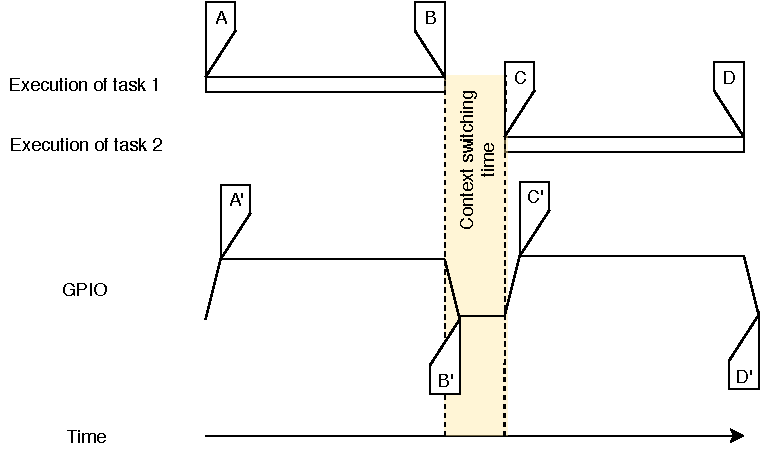
\includegraphics[scale=1]{assets/external-framework-context-switching-time-measurement.pdf}
  \caption{\label{fig:external-framework-context-switching-time-measurement}Measurement of the context switching time with a single GPIO}
\end{figure}

\subsection{Roles}

With the benchmarked board, the PSLab and the computer, we have three devices that we use to compute the context switching time.
The figure \ref{fig:external-benchmarking-framework-schema} shows the connections between the different devices.
To make some clarity, we have defined a specific role to each device.

\subsubsection{The PSLab}
It is the eye of the benchmarking framework.
It watch the benchmarked board through a single GPIO.
It use this port to compute the context switching time using its logical analyser.
It receives its instruction from our computer through UART.

\subsubsection{The computer}
It is the brain of the benchmarking framework.
It is responsible of communicating with both the benchmarked board and the PSLab through the UART protocol.
It is its responsability to coordinate the benchmarked board and the PSLab in order to retrieve the context switching time.
The computer is also the place where all the data are accumulated.

\subsubsection{The benchmarked board}
It runs the RTOS Contiki with our benchmarking framework and our simple application.
It communicate with our computer through UART and with the PSLab using a single GPIO.
Its role is to simply run the application.

\begin{figure}[!ht]
  \centering
  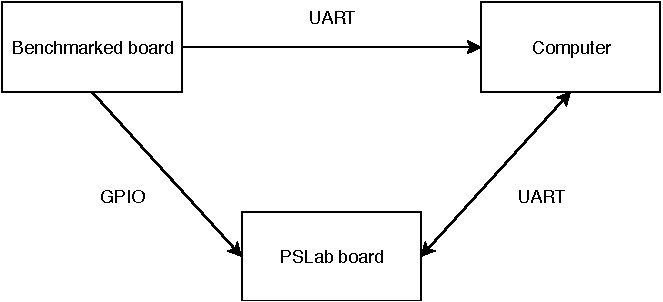
\includegraphics[scale=1]{assets/external-benchmarking-framework-schema.pdf}
  \caption{\label{fig:external-benchmarking-framework-schema}Interaction schema of the devices used in the framework}
\end{figure}

\subsection{Implementation}

In order to implement this third approach, we need to update our simple task, create our framework in Contiki as an app and creating a Python script that will run on the computer and communicate with both the benchmarked board and the PSLab.

% Tout d'abord nous devons définir une sorte de logique ou protocole afin de synchroniser l'ensemble des devices et mesurer efficacement le context switching time.
% 

\begin{figure}[!ht]
  \centering
  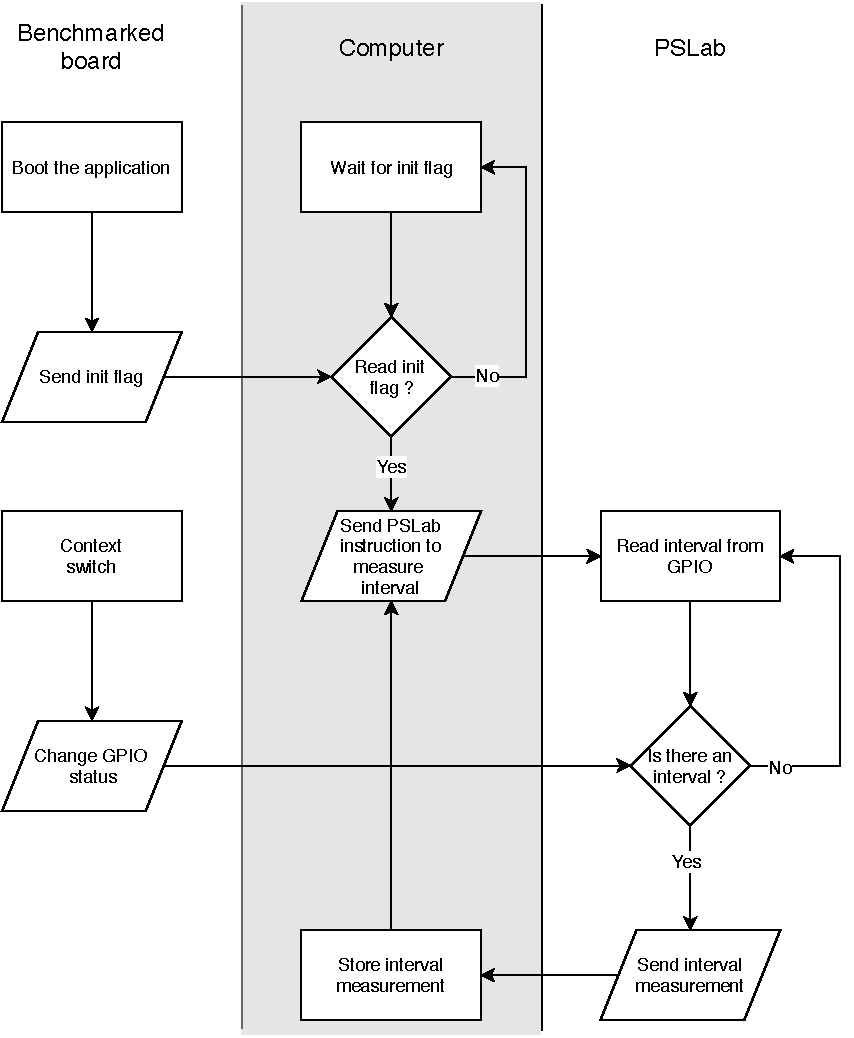
\includegraphics[scale=0.7]{assets/external-protocol.pdf}
  \caption{\label{fig:external-protocol}Schema of the protocol used between the devices}
\end{figure}



